The current document describes the testing procedures adopted in the development of the hazard component of the \gls{acr:oqe}, the open source hazard and risk software developed by the Global Earthquake Model initiative.

Nowadays seismic hazard analysis serves different needs coming from a variety of users and applications.

These may encompass engineering design, assessment of earthquake risk to portfolios of assets within the insurance and reinsurance sectors, engineering seismological research, and effective mitigation via public policy in the form of urban zoning and building design code formulation.

Decisions based on seismic risk results may have impacts on
population, properties and capitals, possibly with important repercussions on our day-to-day life. For these reasons, it is recommendable that the generation of hazard models and their calculation is based on well-recognized, state-of-the-art and tested techniques, requirements that must be reconciled with the need to regularly incorporate recent advances given the progress carried out within the scientific community.

The features described below contribute to fulfill these requirements: %
\begin{itemize}
\item Software should have a modular and flexible structure capable of incorporating new features and - as a consequence - offer users the most recent and advanced techniques.
%
In very general terms, modularity is the level to which a component of a system can be moved, replaced or reused.
%
In software design, modularity means the separation of the software
into smaller independent components that can be implemented, maintained and tested easily and efficiently.
%
\item Software should have and extensive test coverage which captures possible errors and avoids regressions (i.e. unexpected behaviors introduced by new features).
%
Software testing \citep{myers2012} is an important, complex and vast discipline which helps in developing methods and processes aimed at certifying the extent to which a computer code behaves according to the original design intent and user specifications.
\end{itemize}


\begin{figure}[!ht]
\centering
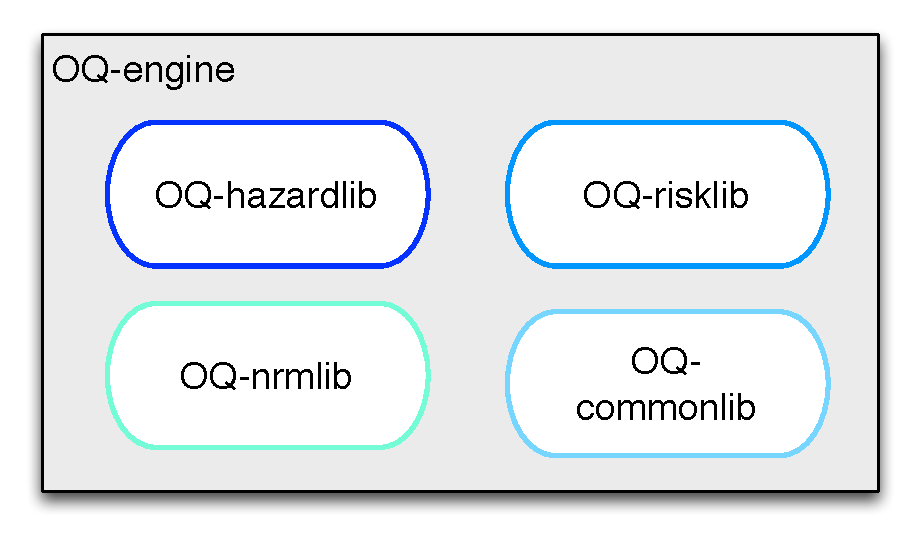
\includegraphics[width=9cm]{figures/oq_engine_structure.pdf}
\caption{A schematic describing the main components of the OpenQuake-engine software.}
\label{fig:oqe-structure}
\end{figure}


The \gls{acr:oqe} includes different levels of modularity. The first is the one separating the engine itself into a number of libraries (see Figure \ref{fig:oqe-structure}), each one containing well identified knowledge, objects and methods (e.g. the OQ-hazardlib  includes objects and methods needed to compute probabilistic seismic hazard and the OQ-risklib contains methods to compute scenario and probabilistic seismic risk).

The second one pertains to the data model adopted in the development of each library as a result of the abstraction process.

According to \citet{berkes2012} scientific software must be:
\begin{itemize}
\item Error proof
\item Flexible and able to accommodate different methods
\item Reproducible and re-usable
\end{itemize}